\documentclass[a4paper,11pt]{article}
\usepackage[margin=2cm]{geometry}
%\usepackage{anysize}
\usepackage[pdftex]{graphicx}
\usepackage{url}
\usepackage{fixltx2e}
\usepackage{listings}
\usepackage{textcomp}
\usepackage{wrapfig}
\usepackage{color}
\usepackage{subfig}
\usepackage{fancyhdr}
\usepackage{newclude}
\usepackage[nodayofweek]{datetime}
\usepackage[small,compact]{titlesec}
\usepackage[pdfborder=0]{hyperref}
\longdate

\setlength{\parskip}{11pt} 
\setlength\parindent{0pt}

\pagestyle{fancyplain}
\fancyhf{}
\lhead{\fancyplain{}{Machine Learning CBC}}
\rhead{\fancyplain{}{\today}}
\cfoot{\fancyplain{}{\thepage}}


\title{395 Machine Learning\\\Large{--- Assignment 3 ---}}
\author{Group 7\\Porfyrios Vasileiou, Afxentios Hadjiminas, John Flanagan.\\
       \{pv311, ah2411, jf311.\}@doc.ic.ac.uk\\ \\
       \small{CBC helper: Ioannis Marras}\\
       \small{Course: CO395, Imperial College London}
}


\begin{document}
\maketitle

\section{Implementation}
The scope of this coursework is to acquire knowledge about how neural networks work in Matlab and how can they be trained for classifying. Furthermore, it was required to find the best parameters for the network that will maximise the results. Parameters such as the training function, learning rule and rate, activation function and more. It is also required to compare the performance of multiple single output networks instead of one single multiple output network. The performance is again computed using 10-Fold Cross-Validation with the same approach as for the decision trees. The whole examples table is divided each time into test and train sets with the test set occupying the 10\% of the total examples. Each fold, the actual and predicted labels are found and in the end we calculate the average confusion matrix. Using the matrix we can then calculate the average precision, recall and F1 measure. The networks are created using the function \emph{feedforwardnet()}where we assign the number of hidden layers and the training function. In the last assignment each row was an example with the attributes assigned to the columns. For neural networks each column is a different example and the attributes lay in the rows. For this transformation we use the given function \emph{NNdata(x, y)} that is provided. 


\section{Network Parameters}
For deciding the best network for the scope of this coursework experiments were made with various network parameters. For instance networks were tested with different numbers of hidden layers, neurons per layer and learning rate. Additionally we trained the network with various transfer functions and training functions in order to find the best combination that outputs better results. This procedure took a lot of time, however it was essential to identify the best network configuration. These parameters are discussed thoroughly in the next section.

\subsection{Training Function}
The most important parameter of the network is the training function. After testing a number of these functions it was found that \emph{trainscg} and \emph{trainbr} were the ones with the best performance and minimum average error between 4\% and 8\%. A reason for this is that they do a very good job with early stopping and regularisation. However in most cases \emph{trainscg} had slightly better results and was significantly faster. Other training functions that were tested were \emph{trainlm}, \emph{traingd} and \emph{traingdm}. \emph{trainlm} achieved 9\% average error when using 2 hidden layers of 20 neurons each whereas \emph{traingd} and \emph{traingdm} both produced relatively high average errors for 1 and 2 hidden layers between 15\% and 40\%.

\subsection{Learning rate}
Learning rate is another important parameter that must be set in order to achieve good results. Values between 0.01 and 0.1 were used as recommended. It was observed that using high rates was producing bad results and same applied for too low rates. After some testing, it was decided to use 0.05 as the learning rate because it produced the lowest error and hence better results.

\subsection{Transfer Function}
For deciding the best transfer function we tested \emph{tansig}, \emph{logsig} and \emph{purelin}. These tests were made for both network approaches. The worst results came from using purelin as we observed overfitting and early stopping was not efficient. We achieved the best results with \emph{tansig} where we received the minimum error of the three functions. It was also found that \emph{logsig} was the faster with slightly worse results than \emph{tansig}.

\subsection{Epochs}
Since early stopping and regularisation methods were applied, the number of epochs seemed to never reach or pass 100. Therefore it was set to 100 that was more than enough for this coursework.

\subsection{Topology}
For deciding the appropriate network topology we experimented with different numbers of hidden layers as well a different number of neurons for each layer. After producing the average error for each case, it was decided to use 1 or 2 hidden layers. For 1 hidden layer use 30-50 neurons whereas for 2 hidden layers we assign 30 neurons for each layer. Using more hidden layers produced lower quality results as the complexity of the network and training time increased. In addition using many hidden layers increases the probability of overfitting and over training. 	

1 hidden layers
(10):0.07
(35):0.05
(45):0.06
(50):0.02
(60):0.04
(100):0.14

2 hidden layers 
(10 10): 0.14
(30,30): 0.04  

3 hidden layers 
(10 10 10):0.20

\section{Regularization Methodology}
The main problem we faced during the training of the Neural Network was the overfitting. The network has been trained with a very low error rate, however when the new data was included, the performance was very bad with a high error rate. That�s because the network memorized the samples from the training set but it was not able to adapt to the new situation, resulting overfitting. In order to solve this problem by improving the generalization, two methods have been adopted.

\subsection{Modified Performance Function}
In this method, the performance function has been changed. The default performance function \emph{MSE} is the mean sum of squares of the network errors on the training set. To improve the generalization, a term that consists of the mean of the sum of squares of the network weights and biases has been added to the \emph{MSE} resulting in the \emph{MSEREG} function. Using this performance function \emph{net.performFcn = msereg} the neural network has smaller weights and biases, and as a result the network is less likely to overfit and its outcome is smoother.

\subsection{Bayesian Regularisation}
Another way to improve the generalization is through the regularisation of small data sets with Bayesian Regularisation. The \emph{trainbr} function, which implements the Bayesian regularisation was tested for training the network. However, after testing the team decided that the performance of the network using the training function \emph{trainscg} along with the performance function \emph{msereg} is better when compared to the network with the \emph{trainbr} function.

\subsection{Early Stopping}
The second method that has been used to avoid overfitting is stopping the training of the network at an earlier point. For this purpose, Matlab offers modification option on the training function. In the specific neural network the following training parameters of the \emph{trainscg} has been set up. Firstly, the \emph{net.trainingParam.goal} has been set up in order to stop the training when the network has achieved classifying correctly 99\% of all examples. Secondly, the \emph{net.trainParam.min\_grad} which is responsible for stopping the training when the gradient of the network performance reaches a certain minimum has been used with the value 0.01. This value was chosen so that the training stops when the error rate decreases by a small amount, but not smaller than 0.01.  Lastly, the parameter \emph{net.trainParam.epochs} was chosen to have the value of 100 maximum epochs, based on the experiment results which have been discussed in the previous section.

\section{Validation Results}
Below are the final average Confusion Matrices, Recall, Precision rates and the F1 measure of both network approaches. The network parameters for both types of networks:

\begin{description}
  \item[Training Function] \emph{trainscg}
  \item[Hidden Layers] 2
  \item[Neurons] [30 30]
  \item[Epochs] 100
  \item[Learning Rate] 0.05
  \item[Goal] 0.01
  \item[Min Grad] 0.01
  \item[Transfer Function] \emph{tansig}
  \item[Perform Function] \emph{msereg}
\end{description}

\pagebreak
\subsection{Performance(F1 Measure) per fold}
These graphs show the mean F1 measure computed for each fold

 \begin{figure}[h]                                                               
 \begin{center}                                                                  
           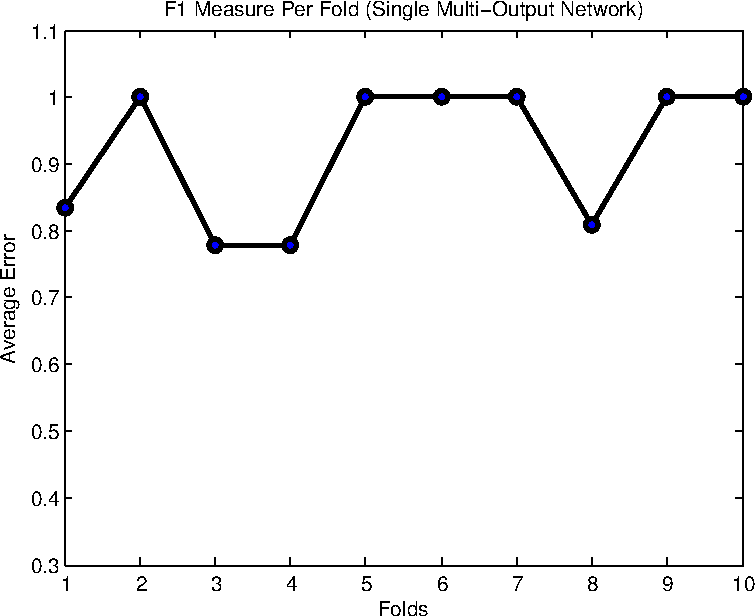
\includegraphics[width=.5\textwidth]{mpfmulti.pdf}                                       
 \end{center}                                                                    
 \end{figure} 
 
  \begin{figure}[h]                                                               
 \begin{center}                                                                  
           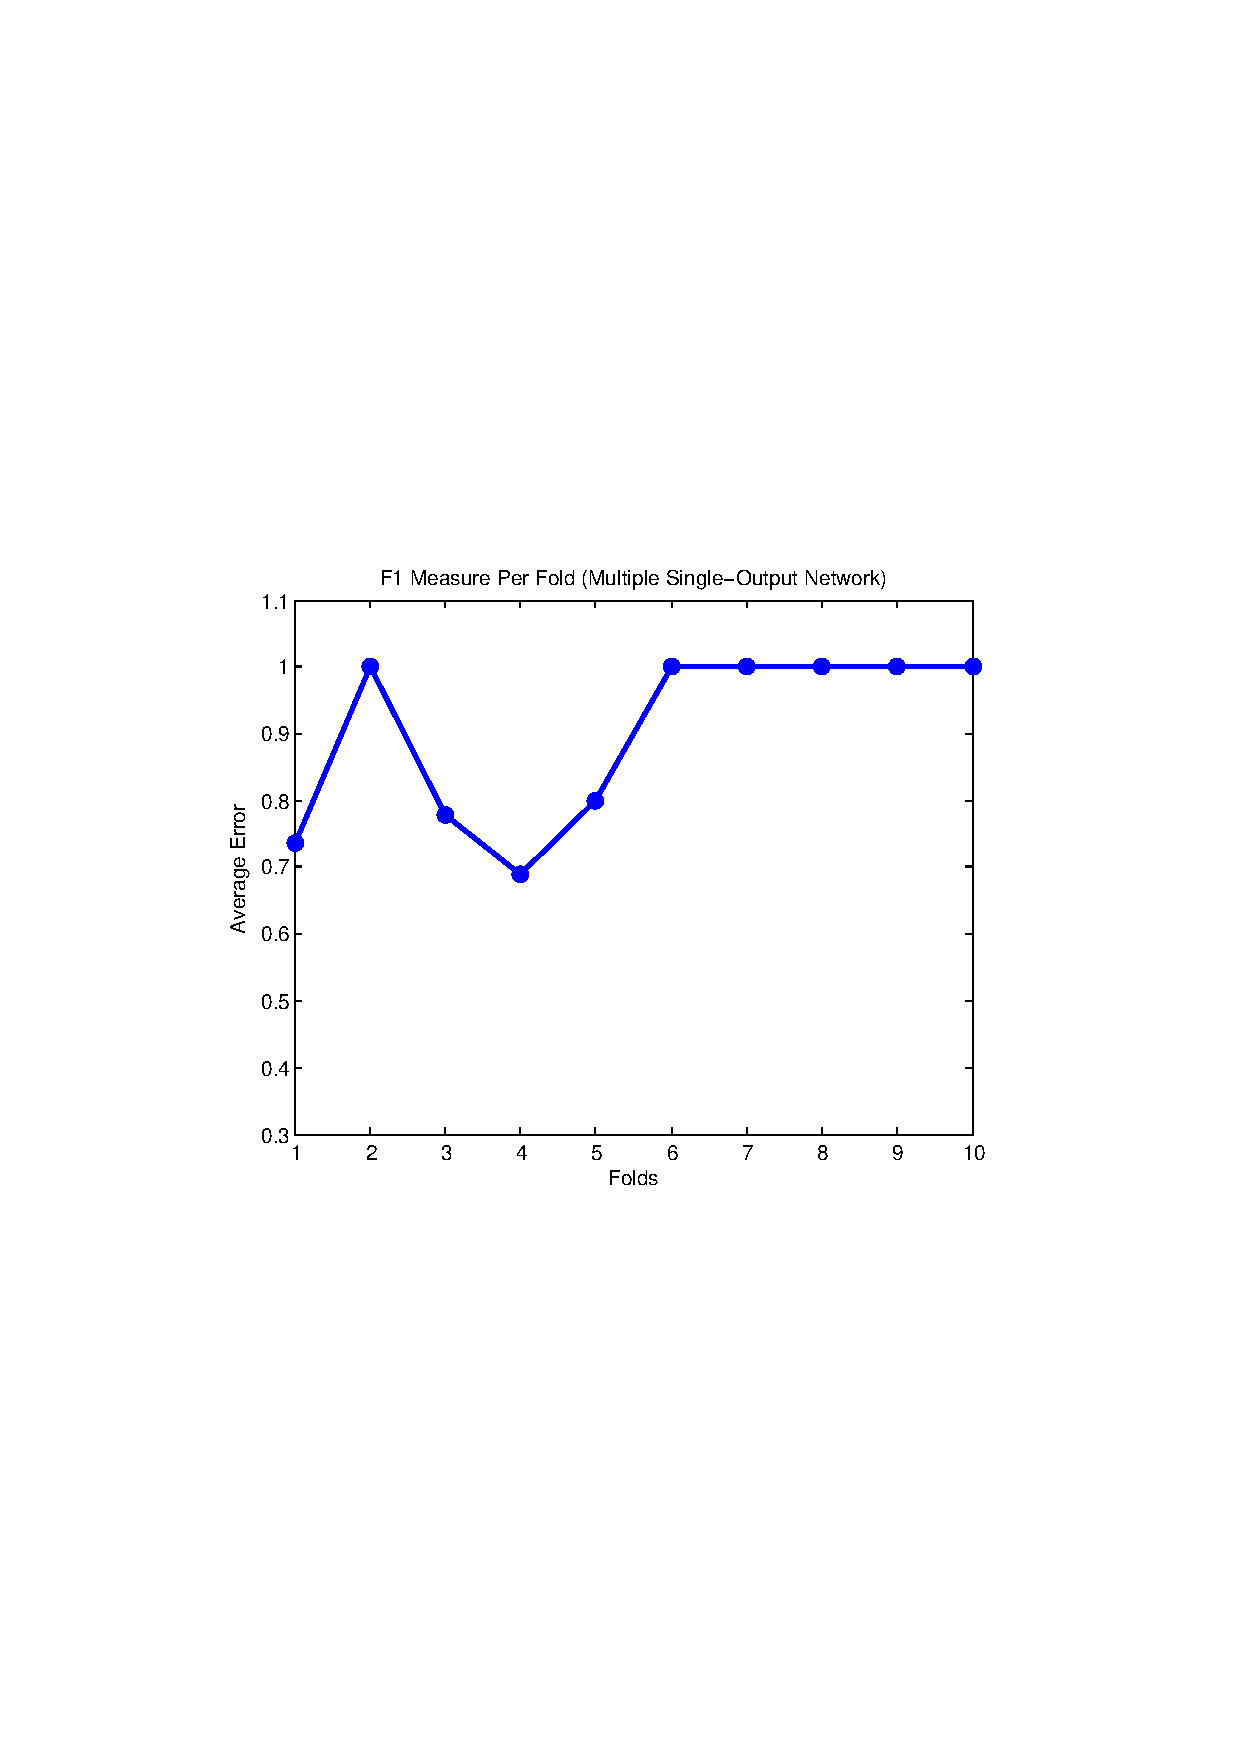
\includegraphics[width=.5\textwidth]{mpfsingle.pdf}                                      
 \end{center}                                                                    
 \end{figure} 


\subsection{10-Fold Cross-Validation Average Results}
                                                              
\begin{center}                                                                  
     \begin{tabular}{ | l || c | c | c | c | c | c | }                           
     \hline                                                                      
           & Anger 1 & Disgust 2 & Fear 3 & Happiness 4 & Sadness 5 & Surprise 6 \\ \hline \hline
         Anger 1 		& 11 & 0 & 0 & 0 & 0 & 0 \\ \hline                               
         Disgust 2 		& 0 & 21 & 0 & 0 & 0 & 0 \\ \hline                            
         Fear 3 		& 2 & 0 & 5 & 0 & 0 & 0 \\ \hline                                
         Happiness 4 	& 0 & 0 & 0 & 24 & 0 & 0 \\ \hline                          
         Sadness 5 		& 0 & 0 & 0 & 0 & 12 & 0 \\ \hline                             
         Surprise 6 	& 0 & 0 & 0 & 0 & 0 & 23 \\ \hline                           
     \end{tabular}                                                               
          \\ One Multi-Output Confusion Matrix.                                         
\end{center}                                                                    
   

                                                               
 \begin{center}                                                                  
 \begin{tabular}{ | l || c | c | c | c | c | c | }                               
     \hline                                                                      
           							& Anger 1 & Disgust 2 & Fear 3 & Happiness 4 & Sadness 5 & Surprise 6 \\ \hline \hline
         Avg Recall 				& 0.9166 & 0.9545 & 0.7142 & 1 & 1 & 1 \\ \hline   
         Avg Precision 				& 0.8461 & 1 & 0.7142 & 1 & 1 & 1 \\ \hline
         F\textsubscript{1} Measure & 0.8800 & 0.9767 & 0.7143 &  1.0000 &  1.0000 & 1.0000 \\ \hline
     \end{tabular}                                                               
     \\ One Multi-Output evaluation results    
 \end{center}                                                                    

\begin{description}
	\item[F\textsubscript{1} Measure Mean] 0.928504983388705
	\item[Avg Error] 0.04
\end{description}

                                                             
\begin{center}                                                                  
     \begin{tabular}{ | l || c | c | c | c | c | c | }                           
     \hline                                                                      
           & Anger 1 & Disgust 2 & Fear 3 & Happiness 4 & Sadness 5 & Surprise 6 \\ \hline \hline
         Anger 1 		& 11 & 0 & 1 & 0 & 0 & 0 \\ \hline                               
         Disgust 2 		& 1 & 21 & 0 & 0 & 0 & 0 \\ \hline                            
         Fear 3 		& 2 & 0 & 5 & 0 & 0 & 0 \\ \hline                                
         Happiness 4 	& 0 & 1 & 0 & 23 & 0 & 0 \\ \hline                          
         Sadness 5 		& 1 & 0 & 0 & 0 & 11 & 0 \\ \hline                             
         Surprise 6 	& 0 & 0 & 0 & 0 & 0 & 23 \\ \hline                           
     \end{tabular}                                                               
     \\ Six Single-Output Confusion Matrix.                                              
\end{center}                                                                    

                                                              
 \begin{center}                                                                  
 \begin{tabular}{ | l || c | c | c | c | c | c | }                               
     \hline                                                                      
           							& Anger 1 & Disgust 2 & Fear 3 & Happiness 4 & Sadness 5 & Surprise 6 \\ \hline \hline
         Avg Recall 				& 0.9167 & 0.9545 & 0.7143 & 0.9583 & 0.9667 & 1 \\ \hline   
         Avg Precision 				& 0.7333 & 0.9545 & 0.8333 & 1 & 1 & 1 \\ \hline
         F\textsubscript{1} Measure & 0.8148 & 0.9545 & 0.7692 &  0.9787 &  0.9565 & 1 \\ \hline
     \end{tabular}                                                               
     \\ Six Single-Output evaluation results                                                                                               
 \end{center}                                                                    


\begin{description}
	\item[F\textsubscript{1} Measure Mean] 0.9123
	\item[Avg Error] 0.06
\end{description}


\section{Single Output Vs Multi Output Networks}
For this assignment we were instructed to approach the problem with two different types of networks. The first one was to create one network that produces six outputs of 0 and 1 each that represent the emotion. For example the output 001000 classifies the example to the third emotion. The other approach was to create a single-output network for every emotion(label) and join the results in the end.
To test more thoroughly the performance of the two approaches we created a script to run the evaluation function that returns the average error for 5 times. This means that the 10-Fold Validation was performed 5 times. The average error returned for both networks was 0.04 for the multi-output network whereas for the single-output networks was slightly higher at 0.06. Additionally the performance(F1 measure) was higher than 9 in both cases with the multi-output network outperforming the single-output approach in terms of f1 measure by 0.01.

Firstly training six single-output networks takes a lot more time than the one multi-output network. Aside from the computational efficiency, the multi-output network suits better in the pattern recognition problem because in this case the six tasks are related, they are all about emotion recognition. The six singe-output networks would be better in the case where the tasks weren�t related at all, for example in the case when one output was about character recognition and another was about emotion recognition.

\end{document}
